\problemname{Find the Box}
Maj is a robotics researcher who works at Lund University.
She has learned about a valuable treasure in the cellar of the university.
The treasure is in a box located in an empty room deep underground.
Unfortunately, Maj cannot just go and look for the box. It is very dark in the
cellar and going there with a light would raise suspicion. Her only way to
find the treasure is to remotely control a robot vacuum cleaner that inhabits the cellar.

The cellar is represented as an $H \times W$ grid, where the rows are numbered from $0$ to $H-1$ (top to bottom) 
and the columns are numbered from $0$ to $W-1$ (left to right), meaning that the top left cell is $(0, 0)$
and the bottom right cell is $(H-1, W-1)$.
The box with the treasure is in some unknown cell, other than the cell $(0,0)$.
Every night, the robot vacuum cleaner starts in the top left corner and moves around the cellar.

Each night, Maj can give the robot a sequence of instructions on how it should move in the form of a string consisting of characters 
`\verb!<!', `\verb!>!', `\verb!^!' and `\verb!v!'.
Formally, if the robot is standing on cell $(r, c)$ that is unblocked on all sides, `\verb!<!' moves the robot left to cell $(r, c-1)$, 
`\verb!>!' moves the robot right to cell $(r, c+1)$, `\verb!^!' moves the robot up to cell $(r-1, c)$, and `\verb!v!' moves the robot down to cell $(r+1, c)$.

The cellar walls are solid, so if the robot attempts to move outside the grid, nothing will happen.
The box is also solid, and cannot be pushed. At the end of each night, the robot will report its location, and go back to the top left corner.

Time is of the essence, so Maj decides to find the box in as few nights as possible.

\section*{Interaction}
This is an interactive problem.

\begin{itemize}

  \item
Your program should start by reading a line with two integers $H$ and $W$: the height and width of the grid.

  \item
Then, your program should interact with the grader. 
In each round of interaction, you should print a question mark `\verb!?!', followed by a non-empty string $s$ 
consisting of characters `\verb!<!', `\verb!>!', `\verb!^!', `\verb!v!'. 
The length of this string can be at most $20\,000$. 
Then, your program should read two integers $r$ and $c$ $(0 \leq r \leq H-1$, $0 \leq c \leq W-1)$, the location of the robot after executing the instructions. 
Note that the robot always goes back to $(0,0)$ after each query.

  \item
When you know the location of the box, print `\verb|!|' followed by the two integers $r_b, c_b$, the row and column of the box $(0\le r_b \le H-1$, $0\le c_b \le W-1)$. After this, your program must exit without making any further queries. This final output does not count as a query when determining your score.
\end{itemize}


Make sure to flush standard output after issuing a query, or else your program might get judged as Time Limit Exceeded.
In Python, \verb@print()@ flushes automatically. In C++, \verb@cout << endl;@ also flushes in addition to printing a newline; if using printf, use \texttt{fflush(stdout)}.

The grader is non-adaptive, meaning that the position of the box is determined before the interaction begins.

\section*{Constraints and Scoring}
\begin{itemize}
  \item  $1 \leq H,W \leq 50$.
  \item The box will never be located at $(0, 0)$. This means that $H+W \geq 3$.
  \item Each query can consist of at most $20\,000$ instructions.
  \item You can issue at most $2\,500$ queries (printing the final answer does not count as a query).
\end{itemize}

Your solution will be tested on a number of test cases. If your solution fails on \emph{any} of these test cases (e.g. by reporting the wrong box position (Wrong Answer), crashing (Runtime Error), exceeding the time limit (Time Limit Exceeded), etc.), you will receive 0 points and the appropriate verdict.

If your program successfully finds the position of the box in \emph{all} test cases, you will get the verdict Accepted, and a score calculated as follows:
\[\text{score} = \mathrm{min}\left(\frac{100\sqrt{2}}{\sqrt{Q}}, 100\right)\text{ points},\]
where $Q$ is the maximum number of queries used on any test case. Printing the final answer does not count as a query. The score will be rounded to the nearest integer.

In particular, to receive $100$ points, your program must solve every test case using at most $Q=2$ queries. The table below shows some values of $Q$ and the associated score.

\begin{center}
\begin{tabular}{r|cccccccccc}
  $Q$ & 2 & 3 & 4 & 5 & \ldots & 20 & \ldots & 50 & \ldots & 2500\\ \hline
  Score & 100 & 82 & 71 & 63 & \ldots & 32 & \ldots & 20 & \ldots & 3 \\
\end{tabular}
\end{center}

\section*{Testing Tool}
To facilitate the testing of your solution, we provide a simple tool that you can download.
See ``attachments'' at the bottom of the Kattis problem page.
The tool is optional to use, and you are allowed to change it. Note that the official grader program on Kattis is different from the testing tool.

Example usage (with $H=4$, $W=5$, and the hidden box at position $r=2$, $c=3)$:

For Python programs, say \verb|solution.py| (normally run as \verb|pypy3 solution.py|):

    \verb|python3 testing_tool.py pypy3 solution.py <<<"4 5 2 3"|

For C++ programs, first compile it
(e.g. with \verb|g++ -g -O2 -std=gnu++17 -static solution.cpp -o solution.out|)
and then run:

    \verb|python3 testing_tool.py ./solution.out <<<"4 5 2 3"|

\section*{Example}

Consider the sample test case. The grid has height $H = 4$ and width $W = 5$, and the box is at position $(r,c) = (2,3)$. 
The figure below shows the robot's path when following the instructions of the first query `\verb!? vv>>>>>><^^^^^>!', 
which results in the robot ending up at position $(r,c) = (0,2)$. 
Before the second query, the robot will go back to the top left corner $(0,0)$ again. Then the solution issues another query
`\verb!? >>>>>>>>vvvvvvvvvv!' for which the robot ends up in the bottom right corner $(r,c) = (3,4)$. 
Now the solution decides to guess the answer, by writing `\verb|! 2 3|', which is the correct position of the box.

\begin{figure}[h]
  \centering
  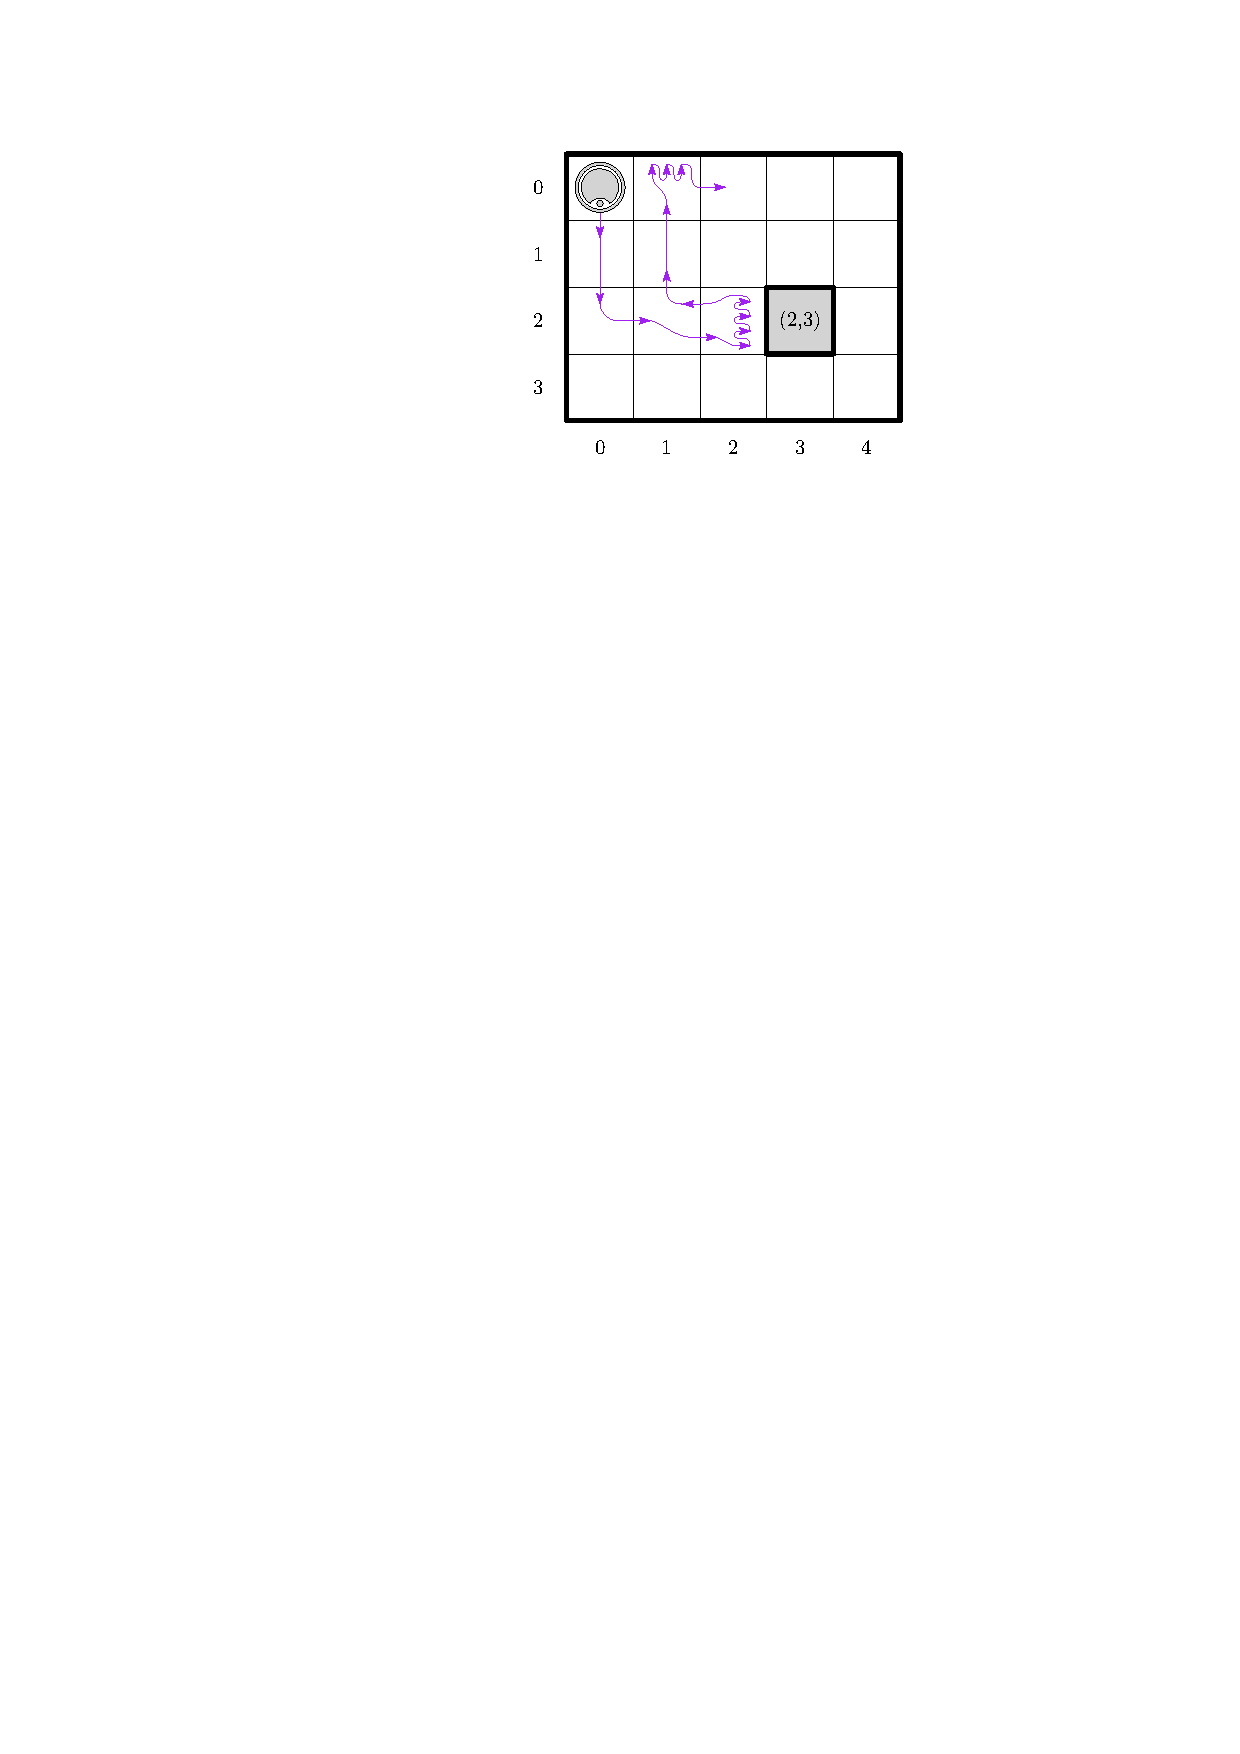
\includegraphics[width=0.6\textwidth]{sample_illustration}
\end{figure}
